\subsection{Golgi}
    Golgi apparatus (or Golgi, or Golgi complex) is another organelle inside the cell that packages proteins into membrane-bound vescicles, that will be exported from the cell. Golgi is located also near the nucleus and ER as well, it is even called a perinuclear body. This location is explained by the bilogical processes: after a protein comes out of the ER, it goes into the Golgi for further processing (\cite{golgi}). The staining of Golgi apparatus has turned out to be the most difficult of all. Two antibodies were tried out for stating here, however both of them resulted in a low signal-to-noise ratio. Many images were underexposed, and the density of the cells after their fixating was pretty low. The hypothesis why this was the case was that the choice of target protein in Golgi to which anti body can bind to was not the best. Golgi appartus is a difficult target even having a fluorescence imaging with high signal-to-noise ratio (lowest scores among all cell organelles in state-of-the-art \cite{Cheng_2021} paper were achieved exactly on Golgi).
    \subsubsection{Preprocessing}
        One can see an example of how Golgi fluorescence staining looks like in Figure \ref{fig:golgi-enhancement}. It is evident that there is a lighter foreground fluorescence and a bit darker one in the background. A true Golgi signal here is considered to be only the lighter part of fluorescence lightning. The light gray background present here is called a non-specific fluorescence lightning. It comes from the cell itself, and might occur when the antigen is impure and contains antigenic contaminants (\cite{Borek_1984}). And brightness of it may vary due to longer or shorter exposure times. 

\begin{figure}[htb]
	\begin{center}
		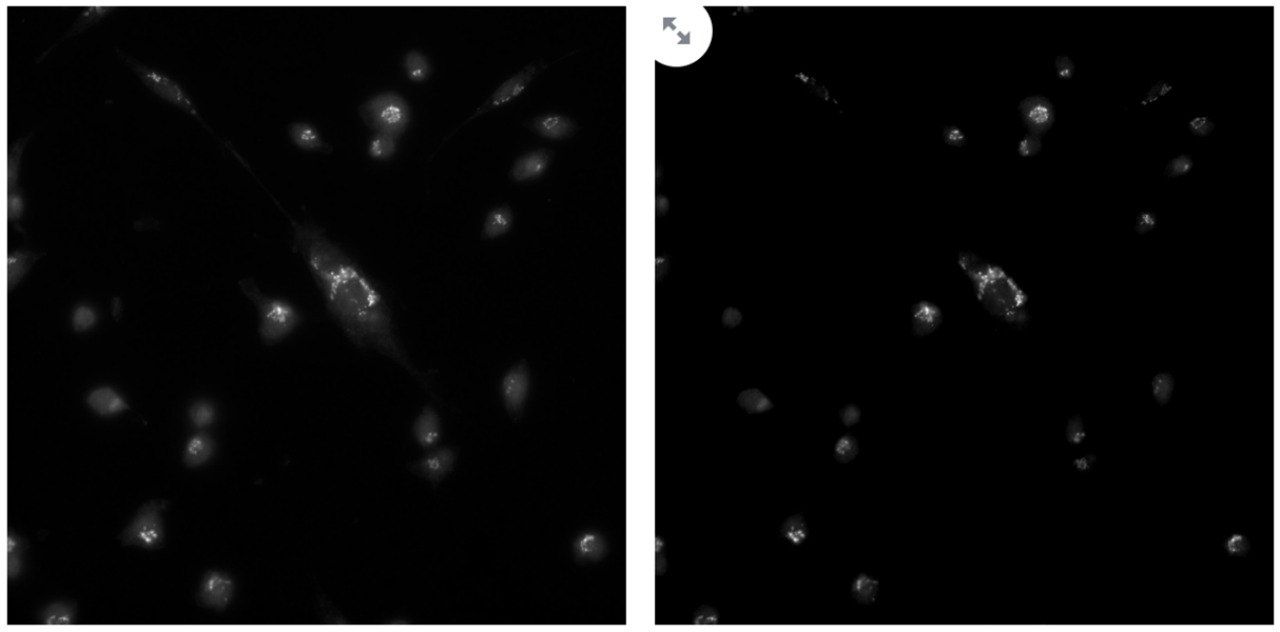
\includegraphics[width=0.5\linewidth]{bilder/enhancement.jpg}
		\caption{Golgi enhancement: left --- original signal, right --- enhanced image}\label{fig:golgi-enhancement}
	\end{center}
\end{figure}

Having such a non-specific fluorescence background has two challenges for training:
\begin{itemize}
    \item The relative area of the background fluorescence is bigger than the area of Golgi themselves. Therefore quite a big part in the loss during training will be dedicated to teaching model to restore this background fluorescence instead of the Golgi itself.
    \item It introduces difficulties during the post-processing of the predictions. As well as for nuclei, the mask of the predicted Golgi apparatus is needed for further evaluation of the downstream metrics. Using the same algorithm for post-processing segmentation that was used for nuclei, the mask of the Golgi Apparatus will consider the background noise to be relevant, although this is an unwanted behavior.
\end{itemize}

On the left of Figure \ref{fig:golgi-enhancement} one can see the original ground truth image and on the right --- the images after the background was substracted. One of the great background subtraction algorithms is the rolling ball algorithm which is described below.

Additionally, all of the crops used for training were filtered base on the amount of background they contain. Without filtering the crops that contain a lot of background, a big portion of a dataset would be black crops only, which creates very strong class imbalance.

        \paragraph{Background removal algorithms}
            \label{par:background-removal}
            The rolling ball algorithm was introduced by \cite{Sternberg_1983} and is still widely used for processing medical and biological data. The idea of this algorithm is based on morphological opening of the image. 

\begin{definition}[Morphological opening]
	Morphological opening is an operation in image processing, when an image is first eroded and then dilated using the same structuring element. 
\end{definition}

Morphological opening is helpful for removing noisy elements, thin lines, while preserving bigger objects in the image (\cite{morph_open}).

A structuring element is an analog of a kernel in image processing. It is a matrix of zeros and ones (true and false), where ones represent the elements that will be used to perform the morphological operation and others will be ignored (see an example in Figure \ref{fig:rolling-ball} [left]). Such a structuring element is applied across the whole input image producing a new image based on the rules of a morphological operation it performs.  

For example, morphological dilation takes a new value of the pixel as the maximum value of its neighbors within the structuring element. Therefore, after this operation, the lines will be thicker and in general objects will appear bigger.

Whereas morphological erosion turns the pixel value into the minimum value of its neighbors within the structuring element. After this operation the floating pixels will be removed and all objects become smaller and thinner.

\cite{Sternberg_1983} has extrapolated the operation of morphological opening from 2D into 3D space. He defines a new interpretation of a 2D image in a 3D world called umbra. Umbra can be described as a 3D plane, where the height of each point is determined by its intesity value.

The structuring element for morphological opening of an umbra has to be then also a 3D object --- in this case a ball. Morphological opening of an umbra is a union of translations of the 3D structuring element that can be entirely contained inside it (see Figure \ref{fig:rolling-ball}). One can imagine the ball freely moving inside the volume constrained by the upper surface of an umbra. The opening then consists of all the pixels that can be reached by the ball. The radius of the ball is a hyper-parameter which has to be tuned.

\begin{figure}[H]
    \centering
    \subfloat[Structuring element]{{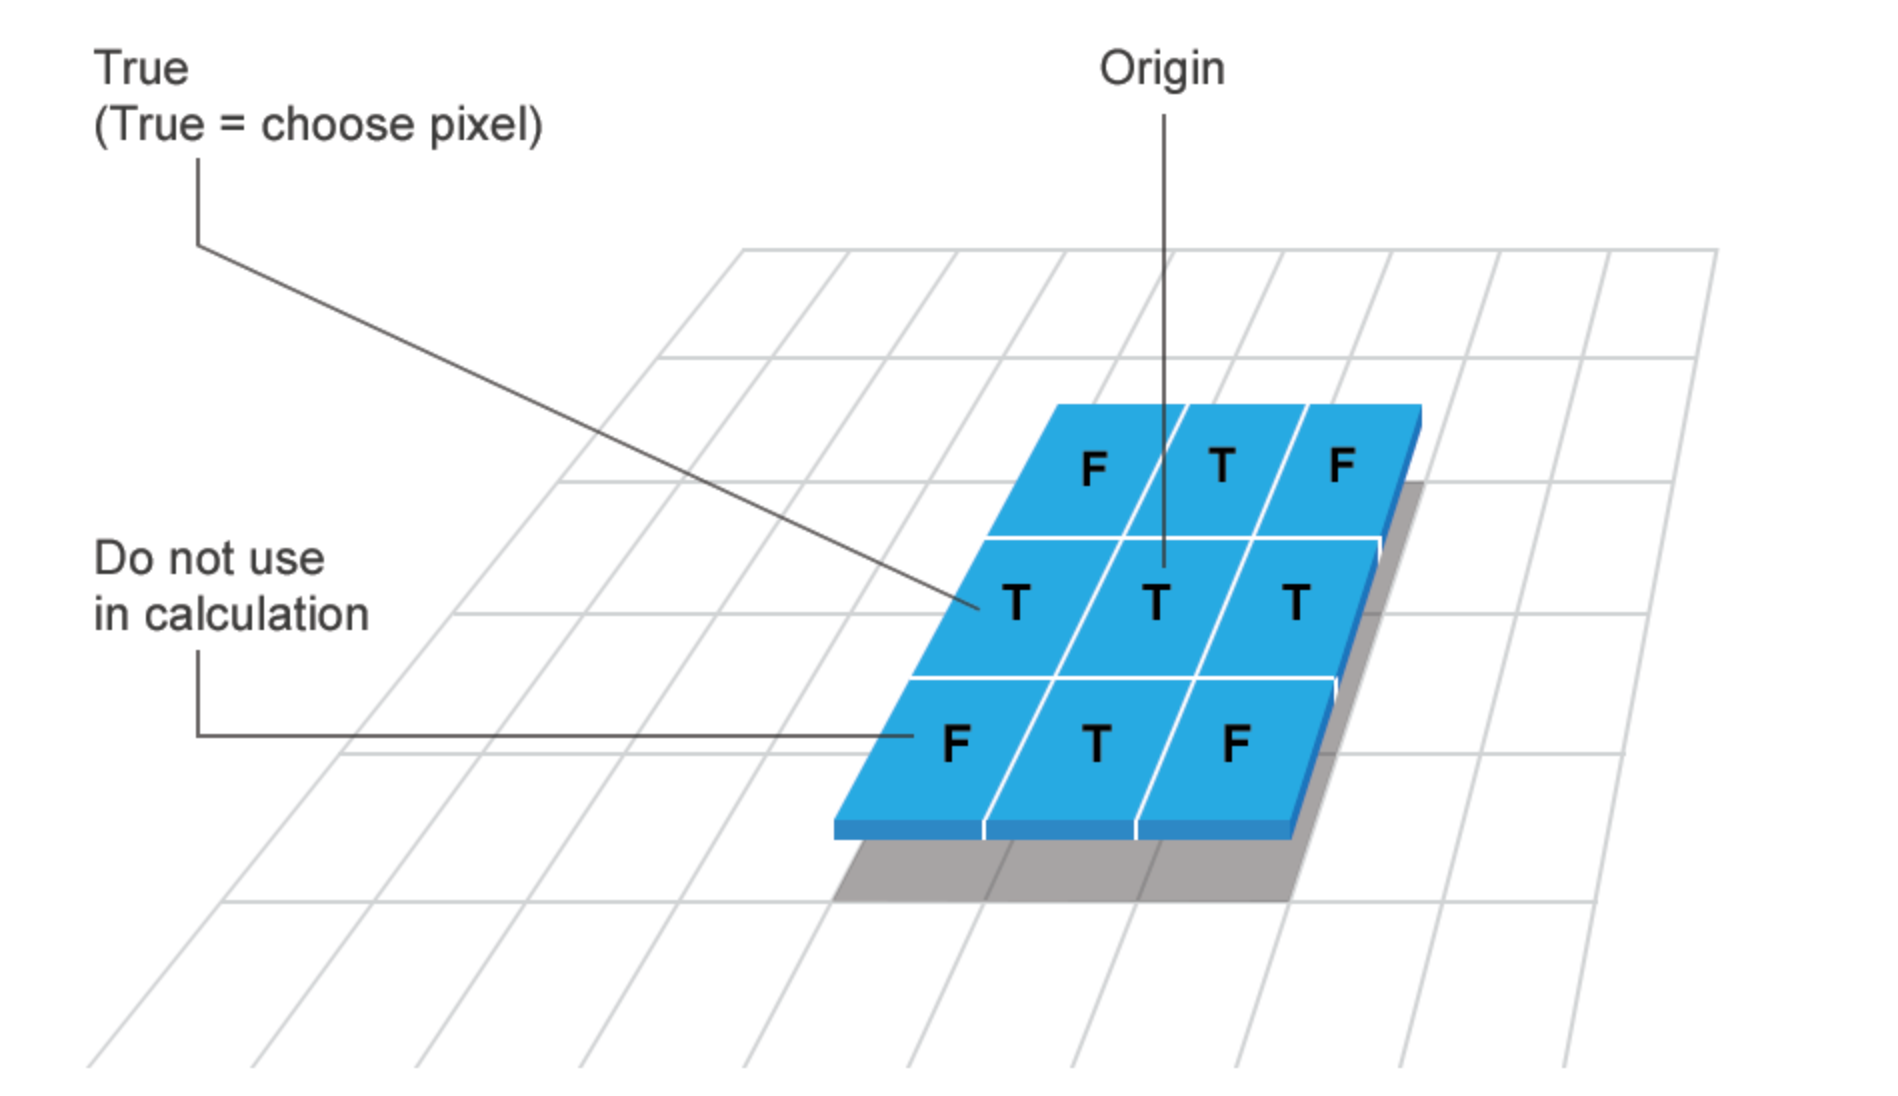
\includegraphics[width=0.3\linewidth]{bilder/structuring-element.png} }}
    \qquad
    \subfloat[Rolling ball]{{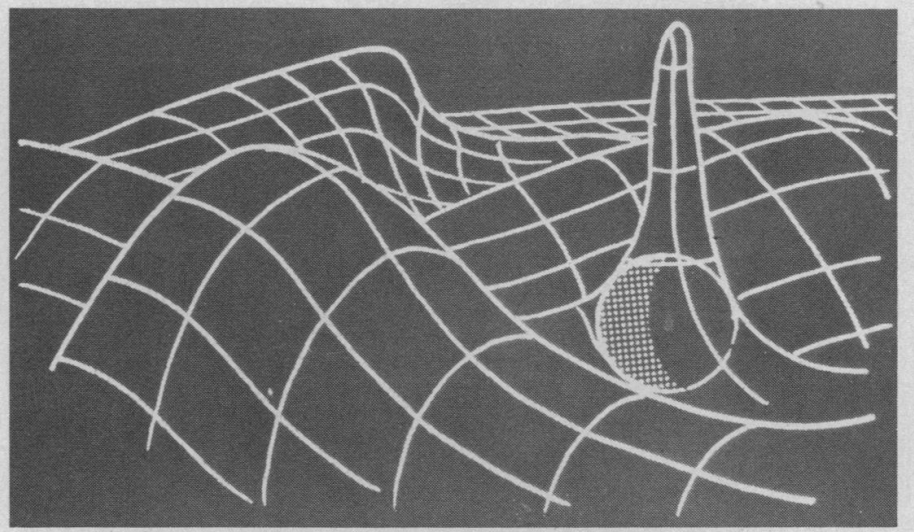
\includegraphics[width=0.3\linewidth]{bilder/rolling-ball.png} }}
    \caption{Background removal}
    \label{fig:rolling-ball}
\end{figure}

Subtracting the background with the rolling ball algorithm unfortunately is still not enough to get a reasonably clean signal of Golgi apparatus from fluorescence imaging, as a lot of background noise will still be present there. In Figure \ref{subfig:vanilla} one can see a fluorescence image preprocessed with a rolling ball algorithm. Let's turn it into a binary image that can be seen in Figure \ref{subfig:vanilla-mask}. 
\begin{figure}[htb]
	\centering
	\begin{subfigure}[b]{0.22\textwidth}
		\centering
		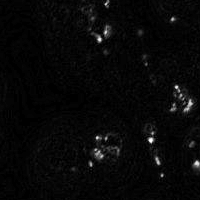
\includegraphics[width=\textwidth]{bilder/preprocessing/crop_golgi_not_full_processed.png}
		\caption{}
		\label{subfig:vanilla}
	\end{subfigure}
	\hfill
	\begin{subfigure}[b]{0.22\textwidth}
		\centering
		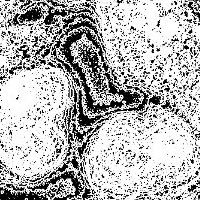
\includegraphics[width=\textwidth]{bilder/preprocessing/crop_golgi_not_full_processed_mask.png}
		\caption{}
		\label{subfig:vanilla-mask}
	\end{subfigure}
	\hfill
	\begin{subfigure}[b]{0.22\textwidth}
		\centering
		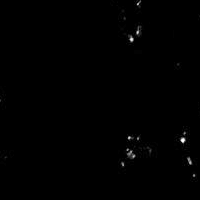
\includegraphics[width=\textwidth]{bilder/preprocessing/crop_golgi_full_processed.png}
		\caption{}
		\label{subfig:clipping}
	\end{subfigure}
	\hfill
	\begin{subfigure}[b]{0.22\textwidth}
		\centering
		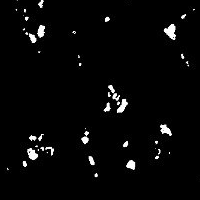
\includegraphics[width=\textwidth]{bilder/preprocessing/crop_golgi_full_processed_mask.png}
		\caption{}
		\label{subfig:clipping-mask}
	\end{subfigure}
	   \caption{(a) Vanilla preprocessing with automatic background removal algorithm only; (b) masked or subfigure (a); (c) Additional clipping of lower intensities after vanilla pre-processing; (d) mask of subfigure (c)}
	   \label{fig:pre-processing-golgi}
\end{figure}
It clearly still contains a lot of background noise of low intensity which was not visible for an eye. In order to get rid of it one could clip lower intensities of the image via the following approach:
\begin{lstlisting}
	import numpy as np
		
	def clip(image):
		minval = np.percentile(image, 90)
		image = np.clip(image, minval, image.max())
		image = (image - image.min()) / (image.max() - image.min())
		return image
\end{lstlisting}

The result of the clipped image and its mask are illustated in Figure \ref{subfig:clipping}, \ref{subfig:clipping-mask} correspondingly. It contains almost no background noise now. Such additional clipping might improve the results slightly.
    \subsubsection{Training and predictions}
        Applying the usual model architecture with PCC loss too train the model to predict fluorescence signal from DIC imaging for Golgi did not bring a good results. Model seems to converge (see Figure \ref{fig:golgi-no-reg-pcc}), however there is no learning happening.
\begin{figure}[H]
	\begin{center}
		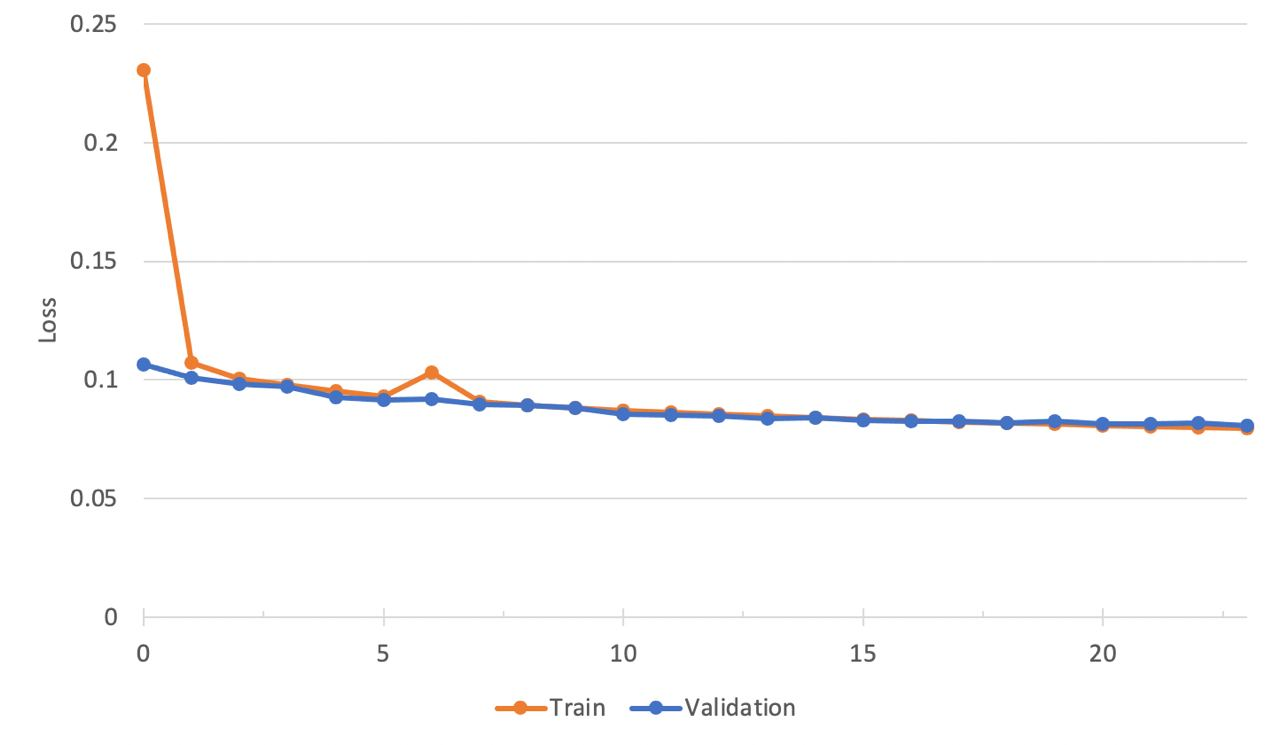
\includegraphics[width=0.8\linewidth]{bilder/golgi/pcc-no-reg.jpg}
		\caption{Straightforward training doesn't work}\label{fig:golgi-no-reg-pcc}
	\end{center}
\end{figure}

This was also depicted in visual predictions where the predicted fluroescence mostly contains dark pixels only (see Figure \ref{fig:golgi-no-reg-pcc-predictions}). Altough it seems that some pattern is hidden behind the dark pixels, visualizing it simply shows that the model picks up on the cell outline itself and does not give any useful information on the location of Golgi. One can see this by normalizing the predicted dark image to the range $[0,1]$ (Figure \ref{fig:golgi-no-reg-pcc-predictions}).
\begin{figure}[htb]
	\begin{center}
		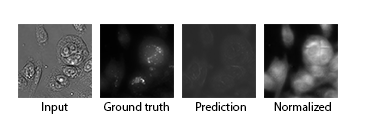
\includegraphics[width=0.8\linewidth]{bilder/golgi/too-dark.png}
		\caption{Training on original data}\label{fig:golgi-no-reg-pcc-predictions}
	\end{center}
\end{figure}

While in Figure \ref{fig:golgi-no-reg-pcc-predictions} only the results of predictions for one crop are presented, it would be interesting to see how the image with combines crops would look like. This is presented in Figure \ref{fig:golgi-no-reg-pcc-predictions-full}. One can notice an interesting pattern there: essentially the model is predicting some signal across the whole cell with a brighter regions in some of them. Yet these regions do not have a correct location wrt to Golgi. Also it is important to keep in mind, that the image of the right in this Figure is a normalized one and a true image is almost fully black.
\begin{figure}[htb]
	\begin{center}
		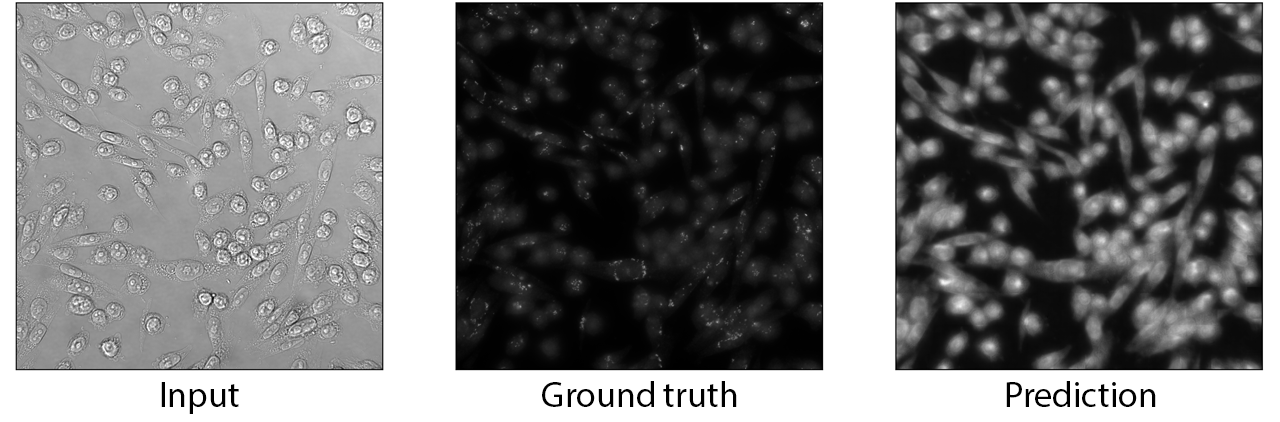
\includegraphics[width=0.8\linewidth]{bilder/golgi/full-img.png}
		\caption{Full size predictions}\label{fig:golgi-no-reg-pcc-predictions-full}
	\end{center}
\end{figure}

This experiment brought a hypothesis that the background removal algorithm might have reduces the signal-to-noise ratio and remove some important fluroescence signal along the way. Therefore an alternative approach of a background removal had been tried, where only enhancing via clipping described above has been applied directly on fluprescence imaging (without using a rolling ball algorithm). This produces images that still have much more non-specific fluorescence background (see Figure \ref{fig:golgi-enhanced-predictions} (second image)), yet this preprocessing alternates the initial image to a much lower extent.

\begin{figure}[htb]
	\begin{center}
		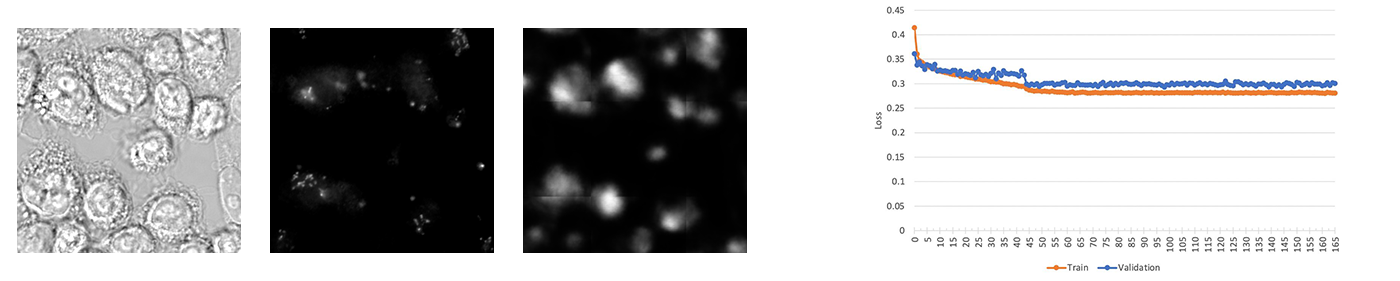
\includegraphics[width=\linewidth]{bilder/golgi/enhanced-crop.png}
		\caption{Training on the enhanced data}\label{fig:golgi-enhanced-predictions}
	\end{center}
\end{figure}
In this case predictions are not completely black anymore, however their quality is still very low. Images used in these training experiments were effectively coming from different staining procedures, using different antibodies, fixation process and microscopy settings. This brought up an idea to train the model on few selective datasets only that were created with the first staining approach only. The preprocessing was chosen as in the previous example --- with the use of enhancement and without rolling ball algorithm as it has shown the best results.

\begin{figure}[htb]
	\begin{center}
		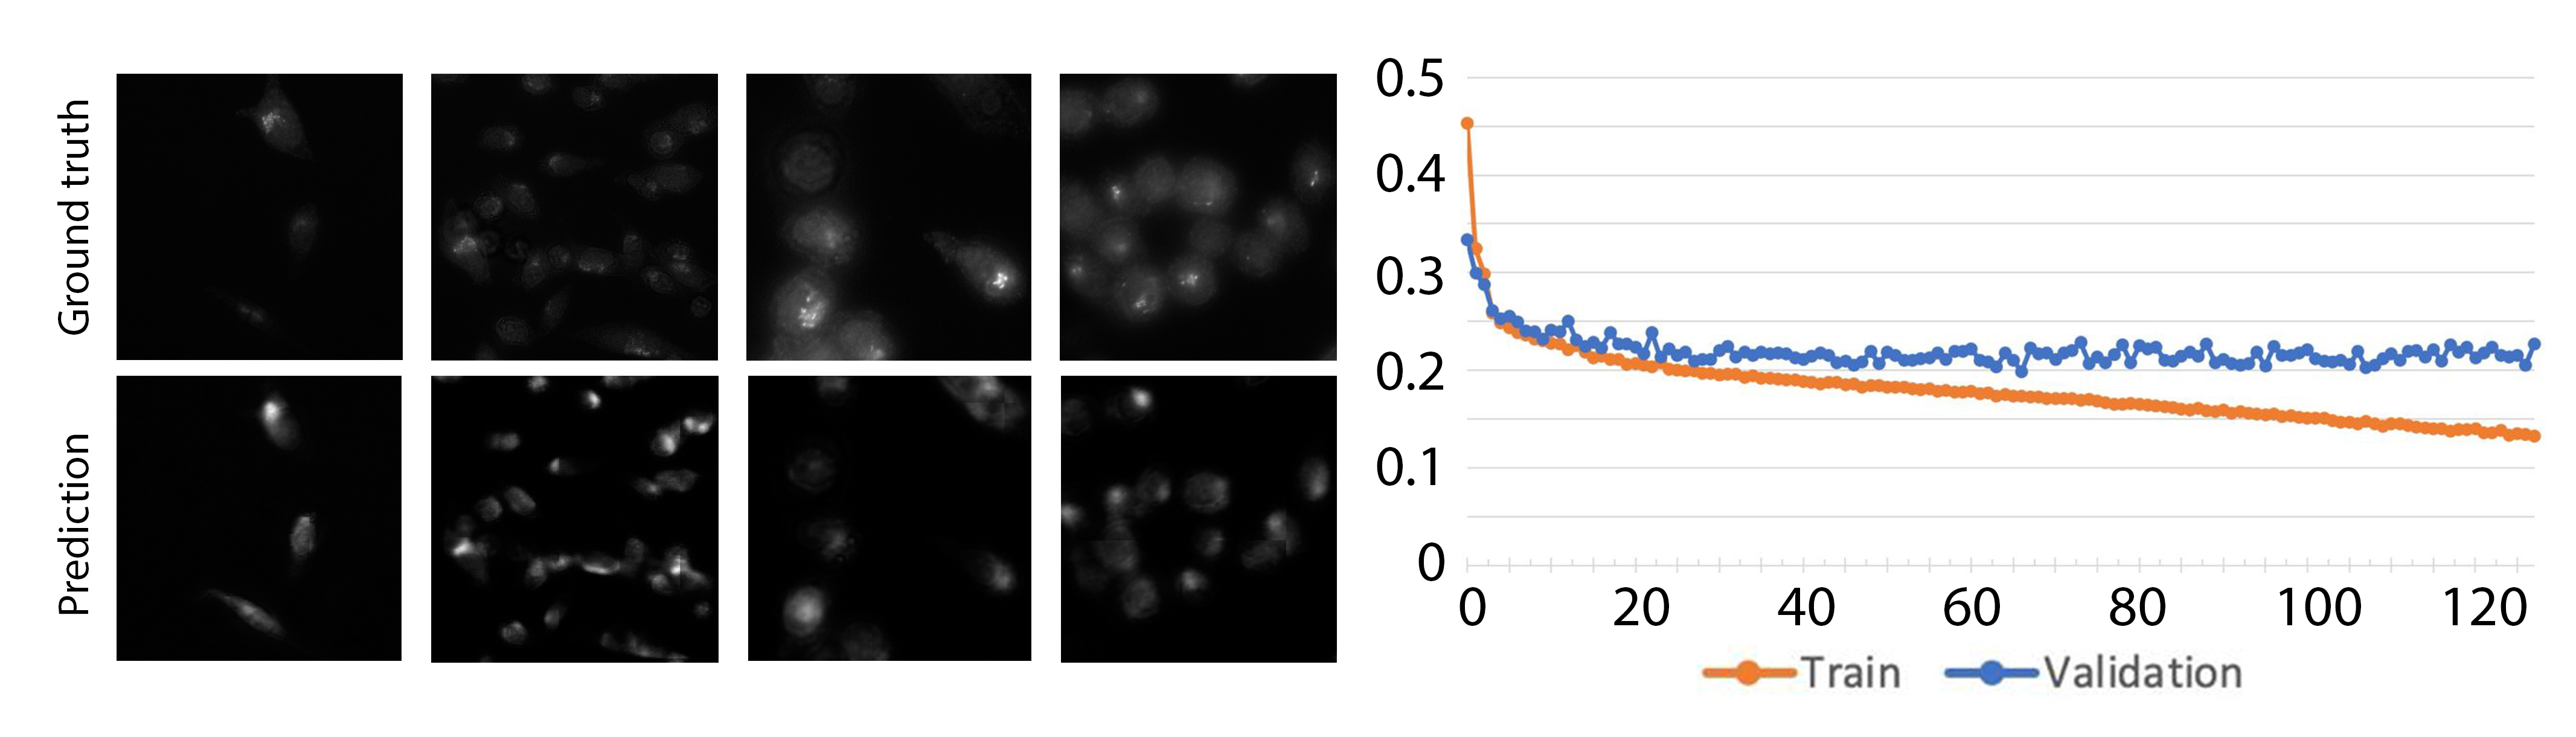
\includegraphics[width=\linewidth]{bilder/golgi/12-13/12-13.png}
		\caption{Small subset of the best staining}\label{fig:12-13}
	\end{center}
\end{figure}

The predictions from this experiment you can find in Figure \ref{fig:12-13}. Due to the stricter filtering and the use of much less data there were much smaller crops which were used for training. In this case only $4251$ crops were used for training and $406$ for validation purposes, which directly led to overfitting after $70$ epochs. However, the predictions did improve visually as well as the loss dropped to $0.19$. Nevertheless the losses from these two experiments should not be compared directly as they were evaluated on two different validation sets. The improvement of the results indicated the careful choice of data samples taken from the same staining approach with the same settings, that does not require a severe preprocessing and already has a high signal-to-noise ratio might help the predictions significantly. There is a potential here for a better regularization of the model trained on the small subset of data. Yet it is clear that the acquisition of a better fluorescence staining is much more crucial here.


    \subsubsection{Alternative ways to improve predictions}
        \paragraph{Asymmetrical losses}
            The earliest learnings from the experiments have shown that the severe class imbalance is present and the model tends to predict mostly pure background --- black images. In order to overcome this an asymmetrical loss can be used during training. Similarly to a weighted loss for a classification problem with class imbalance issue present, a weighted loss for segmentation task can be introduced. In this case different pixels from the prediction will receive a different weight based on some criteria. Yet the use of weights cannot be easily defined for Pearson correlation coefficients, it is possible to use them with MSE loss, because weights coefficients there can be added directly in front of the squared difference between pixels. 
\begin{figure}[H]
	\begin{center}
		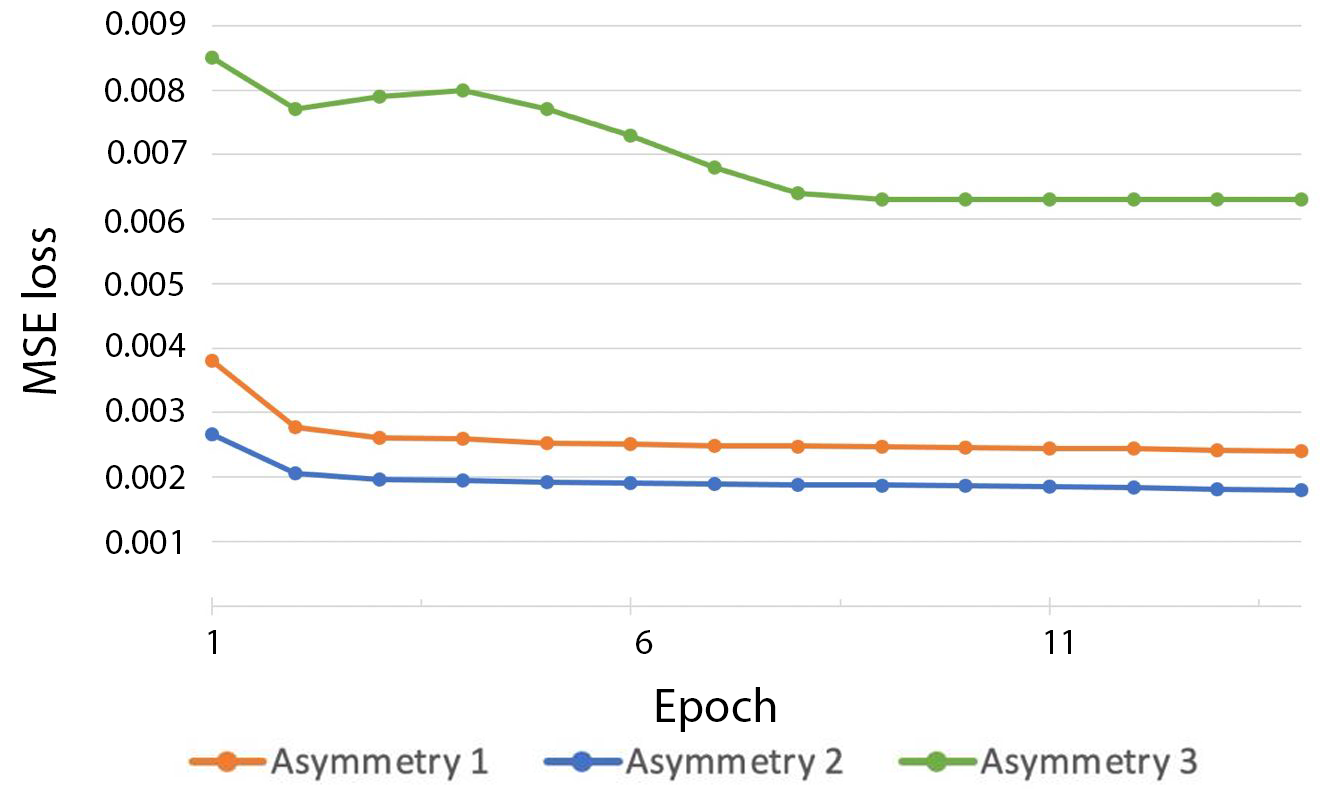
\includegraphics[width=0.5\linewidth]{bilder/golgi/asymmetrical-training.png}
		\caption{Punishing over and under predictions with asymmetrical MSE loss}\label{fig:golgi-asymmetrical-training}
	\end{center}
\end{figure}

Figure \ref{fig:golgi-asymmetrical-training} presents training learning curves from three asymmetrical approaches.

Asymmetry 2 is aimed to punish the errors on bright pixels more: when a model's pixel prediction is higher than a true one the loss will be higher. Yet this loss also encourages the model to underpredict and results in completely black images even though it has the lowest loss.
  \begin{lstlisting}
	  residual = prediction - ground_truth
	  loss = torch.where(residual < 0, residual ** 2, 2 * (residual) ** 2)
	  loss = torch.mean(loss)
	\end{lstlisting}

Asymmetry 1 is aimed to do the opposite and punish an underprediction: when a model's pixel prediction is lower than a true one the loss will be higher. This resulted in slightly brighter images
\begin{lstlisting}
	residual = prediction - ground_truth
	loss = torch.where(residual > 0, residual ** 2, 2 * (residual) ** 2)
	loss = torch.mean(loss)
  \end{lstlisting}

Asymmetry 3 is a stronger version of Asymmetry 1 and it results in 
	\begin{lstlisting}
		residual = prediction - ground_truth
		loss = torch.where(residual > 0, residual ** 3, 20 * (residual) ** 2)
		loss = torch.mean(loss)
	  \end{lstlisting}

All of the approaches above do not bring a significant change in the performance and a mostly black image remained to be an output. Interestingly, punishing underprediction has essentially backfired, as loss then supports an overprediction. Because setting the weights of one class to be smaller amounts to the same as setting the weights of the other class to be larger, and here as a result the model is more likely to overpredict. That is why the second asymmetry has a better loss, even though the logic behind it is not that obvious at first. 

There were other interesting approaches in asymmetrical losses tested that are depicted in Figure \ref{fig:golgi-asymmetrical-training}

1. Adjusting overall brightness. Leads the absence of bright spots and brightness gradients in the prediction. The illumination of the cell becomes uniform across all cells.
\begin{lstlisting}
	loss = loss +  prediction.sum() / ground_truth.sum()
  \end{lstlisting}

2. Adjusting overall brightness with a reversed division. Leads to fully white images as this would minimize the fraction in loss.
\begin{lstlisting}
	loss = loss + ground_truth.sum() / prediction.sum()
\end{lstlisting}

3. Multiplying loss with prediction will result in black images again, however multiplying with the ground truth yields more interesting results. However, the model is pushed to predict average gray color across the entire image for the most part.

\begin{lstlisting}
	loss = MSE(ground_truth, prediction)
	loss = torch.mul(loss, ground_truth)
\end{lstlisting}

4. Multiplying loss with 1 - ground\_truth also results in completely black images as such loss puts more puts more emphasis on the correct prediction of the background.
\begin{lstlisting}
	loss = MSE(ground_truth, prediction)
	loss = torch.mul(loss, 1 - ground_truth)
\end{lstlisting}

5. This improves the asymmetry approach 3, however now the highlighted regions simply include the whole cell.
\begin{lstlisting}
	loss = MSE(ground_truth, prediction)
	loss = torch.mul(loss, ground_truth) + ground_truth.sum() / prediction.sum()
\end{lstlisting}

6. Usual MSE.

7. Usual PCC.

From the experiments it became clear that the best approaches are PCC, pure MSE or MSE with the adjustment of overall brightness.

\begin{figure}[H]
	\begin{center}
		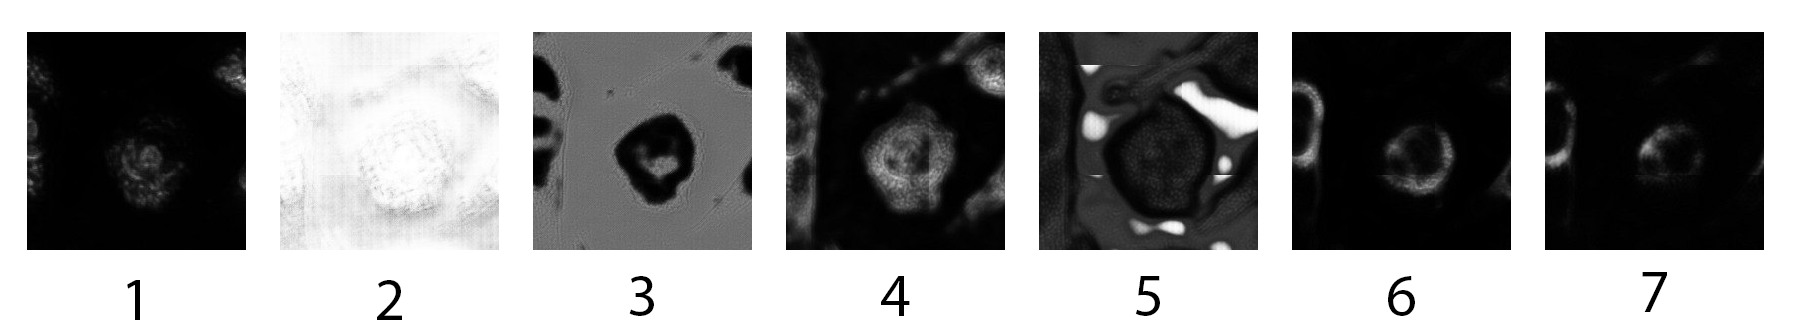
\includegraphics[width=\linewidth]{bilder/golgi/asymmetrical-predictions.png}
		\caption{Results of advanced versions of MSE training}\label{fig:golgi-asymmetrical-predictions}
	\end{center}
\end{figure} 
        \paragraph{Use of gradient in loss}
        \paragraph{Noise reduction methods}
